
%% \begin{figure*}
%%   \vspace{-0.3in}
%%   \centering
%%   \subfloat[\(N=2^2\)]{
%%     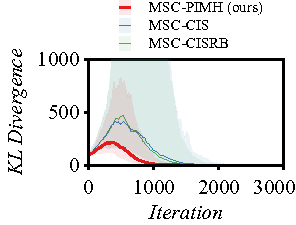
\includegraphics[scale=0.75]{figures/gaussian_01.pdf}
%%   }
%%   \subfloat[\(N=2^4\)]{
%%     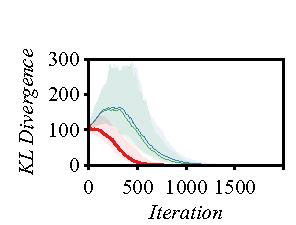
\includegraphics[scale=0.75]{figures/gaussian_02.pdf}
%%   }
%%   \subfloat[\(N=2^6\)]{
%%     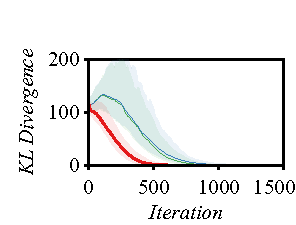
\includegraphics[scale=0.75]{figures/gaussian_03.pdf}
%%   }
%%   \caption{100-D isotropic Gaussian example with a varying computational budget \(N\).
%%     MSC-PIMH converges faster than MSC-CIS and MSC-CISRB regardless of \(N\).
%%     Also, the convergence of MSC-PIMH becomes more stable/monotonic as \(N\) increases.
%%     The solid lines and colored regions are the medians and 80\% percentiles computed from 100 repetitions.
%%   }\label{fig:gaussian}
%%   \vspace{-0.15in}
%% \end{figure*}

\vspace{-0.05in}
\section{Evaluations}\label{section:eval}
\subsection{Experimental Setup}
\paragraph{Implementation}
We implemented MSC with PIMH on top of the Turing~\citep{ge2018t} probabilistic programming framework.
Our implementation works with any model described in Turing, which automatically handles distributions with constrained support~\citep{JMLR:v18:16-107}.
We use the ADAM optimizer by~\citet{kingma_adam_2015} with a learning rate of 0.01 in all of the experiments.
We set a computational budget of \(N=10\) and \(T=10^4\) for all experiments unless mentioned otherwise.

\vspace{-0.1in}
\paragraph{Considered Baselines}
We compare MSC-PIMH against
\begin{enumerate*}[label=\textbf{(\roman*)}]
  \item  MSC using the CIS kernel (\textbf{MSC-CIS},~\citealt{NEURIPS2020_b2070693}), 
  \item  MSC using the CIS kernel with Rao-Blackwellization (\textbf{MSC-CISRB},~\citealt{NEURIPS2020_b2070693})
  \item the adaptive IS method using SNIS as introduced in~\cref{section:ivi_previous} (\textbf{SNIS}),
  \item the reweighted wake-sleep algorithm (\textbf{RWS},~\citealt{DBLP:journals/corr/BornscheinB14}), and  
  \item evidence lower-bound minimization (\textbf{ELBO},~\citealt{pmlr-v33-ranganath14}).
\end{enumerate*}
Specifically, we use automatic differentiation VI (ADVI,~\citealt{JMLR:v18:16-107}) implemented by Turing.

\begin{figure*}
  \vspace{-0.1in}
  \centering
  \subfloat[\texttt{pima}]{
    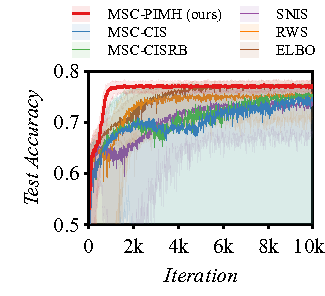
\includegraphics[scale=0.75]{figures/pima_02.pdf}
  }
  \subfloat[\texttt{heart}]{
    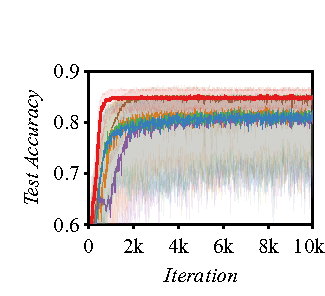
\includegraphics[scale=0.75]{figures/heart_02.pdf}
  }
  \subfloat[\texttt{german}]{
    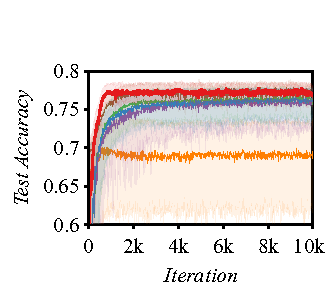
\includegraphics[scale=0.75]{figures/german_02.pdf}
  } \\
  \subfloat[\texttt{pima}]{
    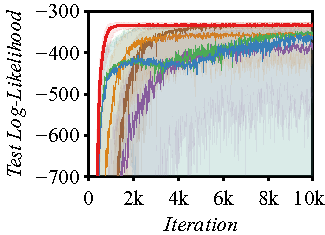
\includegraphics[scale=0.75]{figures/pima_03.pdf}
  }
  \subfloat[\texttt{heart}]{
    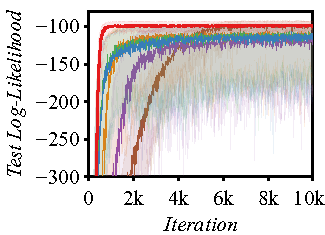
\includegraphics[scale=0.75]{figures/heart_03.pdf}
  }
  \subfloat[\texttt{german}]{
    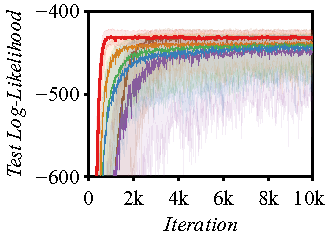
\includegraphics[scale=0.75]{figures/german_03.pdf}
  }
  \caption{Test accuracy and log-likelihood of logistic regression problems.
    The solid lines and colored regions are the medians and 80\% percentiles computed from 100 repetitions.
  }\label{fig:logistic}
  \vspace{-0.2in}
\end{figure*}

\vspace{-0.1in}
\paragraph{Reinterpreting RWS}
The original RWS algorithm assumes that independent samples from \(p(\vz\mid\vx)\) are available, possibly with an additional cost.
%It uses these independent samples for estimating the gradient once every \(K\) steps, and uses SNIS for the rest.
%In our setting, we do not assume that independent samples from \(p(\vz\mid\vx)\) are available.
Since this is not the case in our setting, we reinterpret RWS as alternating between cheap (\textit{sleep update}) and expensive (\textit{wake update}) estimates.
We use respectively use SNIS and HMC for the sleep and wake updates, where we perform the wake update every \(K=5\) steps as originally recommended by~\citet{DBLP:journals/corr/BornscheinB14}.
%HMC shows excellent statistical performance in practice, but is much expensive as it requires multiple gradients \(\nabla_{\vz} p(\vz, \vx)\) for generating only a single samples.

%% \subsection{Isotropic Gaussian}
%% We first perform experiments with an 100-D isotropic multivariate Gaussian distribution.
%% With Gaussian distributions, convergence can be evaluated exactly since their KL divergence is available in a closed form.
%% We compare the performance of MSC-PIMH, MSC-CIS, and MSC-CISRB with respect to the \(N\) (number of proposals for MSC-CIS, MSC-CISRB; number of parallel chains for MSC-PIMH).
%% The results are shown in~\cref{fig:gaussian}.
%% While MSC-PIMH shows some level of overshoot wih \(N=4\), it shows monotonic convergence with larger \(N\).
%% On the other hand, both MSC-CIS and MSC-CISRB overshoots even with \(N=64\).
%% This clearly shows that our PIMH kernel enjoys better gradient estimates compared to the CIS kernel.

\subsection{Hierarchical Logistic Regression}\label{section:logistic}
\vspace{-0.05in}
\paragraph{Experimental Setup}
We now evaluate MSC-PIMH on logistic regression problems.
We consider the Pima Indians diabetes (\textbf{\texttt{pima}}, \(\vz \in \mathbb{R}^{11}\),~\citealt{smith_using_1988}), German credit (\textbf{\texttt{german}}, \(\vz \in \mathbb{R}^{27}\)), and heart disease (\textbf{\texttt{heart}}, \(\vz \in \mathbb{R}^{16}\),~\citealt{detrano_international_1989}) datasets obtained from the UCI repository~\citep{Dua:2019}.
10\% of the data points were randomly selected in each of the 100 repetitions as test data.

\vspace{-0.1in}
\paragraph{Probabilistic Model}
Instead of the usual single-level probit/logistic regression models used in VI, we choose a more complex hierarchical logistic regression model 
%
\begin{equation}
y_i \sim \text{Bernoulli-Logit}\,(p),\;
p \sim \mathcal{N}(\vx_i^{\top}\symbf{\beta} + \alpha,\, \sigma_{\alpha}^2),\;
\symbf{\beta} \sim \mathcal{N}(\symbf{0},\, \sigma_{\beta}^2 \mI),\;
\sigma_{\beta},\,\sigma_{\alpha} \sim \mathcal{N}^{+}(0, 1.0)
\end{equation}
%
where \(\mathcal{N}^+(\mu, \sigma)\) is a positive constrained normal distribution with mean \(\mu\) and standard deviation \(\sigma\), \(\vx_i\) and \(y_i\) are the feature vector and target variable of the \(i\)th datapoint.
The extra degrees of freedom \(\sigma_{\beta}\) and \(\sigma_{\alpha}\) make this model relatively more challenging.

%
\begin{wrapfigure}{r}{0.4\textwidth}
  \vspace{-0.3in}
  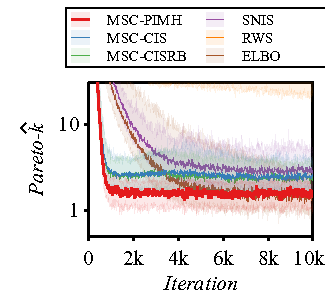
\includegraphics[scale=0.75]{figures/german_01.pdf}
  \caption{Pareto-\(\widehat{k}\) statistics result on \texttt{german}.
    The solid lines and colored regions are the medians and 80\% percentiles computed from 100 repetitions.
    }\label{fig:paretok}
  \vspace{-0.2in}
\end{wrapfigure}
%
\vspace{-0.1in}
\paragraph{Results}
The test accuracy and test log-likelihood results are shown in~\cref{fig:logistic}.
Our proposed MSC-PIMH is the fastest to converge on all of the datasets.
Despite having access to high-quality HMC samples, RWS fails to achieve a similar level of performance to MSC-PIMH.
However, compared to MSC-CIS and MSC-CISRB, it converges faster.
Among the two, MSC-CISRB performs only marginally better than MSC-CIS.
Meanwhile, SNIS is the slowest to converge among inclusive VI methods.
Although much slower to converge, ELBO achieves competitive results.

\vspace{-0.1in}
\paragraph{Inclusive VI v.s. Exclusive VI}
The results of~\cref{fig:logistic} can convey a deceptive conclusion that inclusive and exclusive VI deliver similar results.
However, in the parameter space, they choose very different optimization paths.
This is shown in~\cref{fig:paretok} through the Pareto-\(\widehat{k}\) diagnostic~\citep{NEURIPS2020_7cac11e2, vehtari_pareto_2021}, which determines how reliable are the importance weights computed using \(q_{\vlambda}(\vz)\).
While the test accuracy suggests that ELBO converged around \(t=2000\), in terms of Pareto-\(\widehat{k}\), it takes much longer to converge (about \(t=5000\)).
This shows that, even if their predictive performance is similar, the inclusive VI chooses paths that have better density coverage as expected.

\subsection{Marginal Likelihood Estimation}
%
\begin{figure}[H]
  \vspace{-0.1in}
  \centering
  \begin{minipage}[b]{0.17\linewidth}
    \centering
    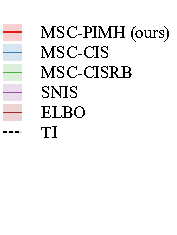
\includegraphics[scale=0.75]{figures/radon_03.pdf}
  \end{minipage}
  \begin{minipage}[b]{0.35\linewidth}
    \centering
    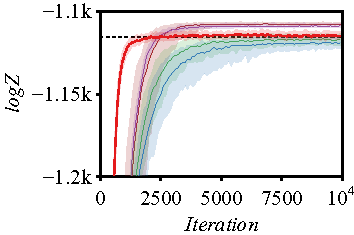
\includegraphics[scale=0.7]{figures/radon_02.pdf}
    \subcaption{\texttt{radon}}
  \end{minipage}
  \begin{minipage}[b]{0.35\linewidth}
    \centering
    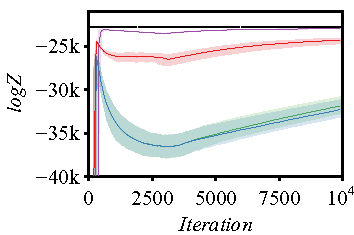
\includegraphics[scale=0.7]{figures/sv_02.pdf}\label{fig:sv}
    \subcaption{\texttt{stock}}
  \end{minipage}
  \caption{Marginal log-likelihood (\(\log Z\)) estimates of considered methods.
    ELBO is omitted in~\cref{fig:sv} as it failed to deliver reasonable estimates.
    The solid lines and colored regions are the medians and 80\% percentiles computed from 100 repetitions.
  }\label{fig:marginal_likelihood}
  \vspace{-0.15in}
\end{figure}
%
\paragraph{Experimental Setup}
We now estimate the marginal log-likelihood \(\log Z\) of a stochastic volatility model (\texttt{stock}, \(\vz \in \mathbb{R}^{2613}\),~\citealt{kim_stochastic_1998}) and a hierarchical regression model with partial pooling (\texttt{radon}, \(\vz \in \mathbb{R}^{175}\),~\citealt{gelman_data_2007}) for modeling radon levels in U.S homes.
For \texttt{stock}, we use 10 years of the S\&P index daily closing price (May 3, 2007, to May 3, 2017).
\texttt{stock} is highly challenging as it is both high dimensional and strongly correlated.
We estimated the reference marginal likelihood using \textit{thermodynamic integration} (TI,~\citealt{gelman_simulating_1998, neal_annealed_2001, lartillot_computing_2006}) with HMC implemented by Stan~\citep{carpenter_stan_2017, betancourt_conceptual_2017}.

\vspace{-0.10in}
\paragraph{Results}
The results are shown in~\cref{fig:marginal_likelihood}.
On \texttt{radon}, MSC-PIMH converges quickly and provides the most accurate estimate.
In contrast, MSC-CIS and MSC-CISRB are much slower to converge.
SNIS and ELBO, on the other hand, overestimate \(\log Z\), which can be attributed to the mode-seeking behavior of ELBO and the small sample bias of SNIS.
On \texttt{stock}, SNIS is unexpectedly the most accurate.
Unfortunately, MSC-PIMH, MSC-CIS, MSC-CISRB all underestimate \(\log Z\).
Nevertheless, MSC-PIMH provides much better estimates than the latter two.
Lastly, we observe that only ELBO fails to converge given the same amount of SGD steps.

%%% Local Variables:
%%% TeX-master: "master"
%%% End:
